\documentclass[crop,dvisvgm,border=4pt]{standalone}

\usepackage{amsmath,amssymb}
  \usepackage{CJKutf8}
  \newcommand{\llbracket}{[\![}
  \newcommand{\rrbracket}{]\!]}
  \usepackage{tikz-cd}
  \usetikzlibrary{arrows.meta,backgrounds,calc,decorations.pathreplacing,fit,positioning,shapes.geometric}
  \newcommand{\pbcorner}{\vcenter{\hbox{\tikz[scale=.22]{\draw[line width=.55pt] (0,1)--(0,0)--(1,0);}}}}

\begin{document}
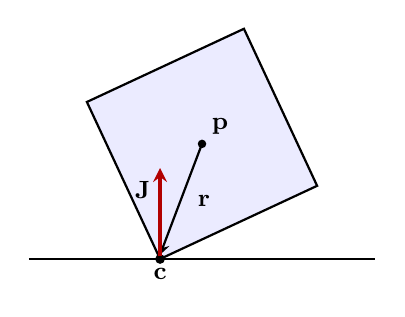
\begin{tikzpicture}[scale=1.1,>=stealth,font=\small]
\fill[blue!8] (-.484,0) -- (1.329,.845) -- (.484,2.658) -- (-1.329,1.813) -- cycle;
\draw[thick] (-.484,0) -- (1.329,.845) -- (.484,2.658) -- (-1.329,1.813) -- cycle;
\draw[thick] (-2,0) -- (2,0);
\fill (0,1.329) circle (1.4pt);
\node[above right] at (0,1.329) {$\mathbf p$};
\fill (-.484,0) circle (1.6pt);
\node[below] at (-.484,0) {$\mathbf c$};
\draw[->,thick] (0,1.329) -- (-.484,.05);
\node[right] at (-.16,.67) {$\mathbf r$};
\draw[->,very thick,red!70!black] (-.484,.03) -- (-.484,1.05);
\node[left] at (-.484,.8) {$\mathbf J$};
\end{tikzpicture}
\end{document}
